\documentclass[a4paper, 14pt]{beamer}
\usetheme{AnnArbor}
\usepackage[T2A]{fontenc}
\usepackage[utf8]{inputenc}
\usepackage[ukrainian]{babel}


\usepackage{caption, hyperref, tempora, authblk, setspace, amsmath, titlesec, geometry, indentfirst, tikz, pgfplots, datetime, cancel, tcolorbox}


\usetikzlibrary{positioning}
\pgfplotsset{width=10cm,compat=1.9}

\onehalfspacing

\hypersetup{
    colorlinks=true,
    linkcolor=orange,
    filecolor=magenta,      
    urlcolor=red,
    pdftitle={Math-Phusics},
}

\urlstyle{same}


\newtcolorbox{mybox}[2][]{enhanced,
before skip=2mm,after skip=2mm,
colback=black!5,colframe=black!50,boxrule=0.2mm,
attach boxed title to top left={xshift=1cm,yshift*=1mm-\tcboxedtitleheight},
varwidth boxed title*=-3cm,
boxed title style={frame code={
\path[fill=tcbcolback!30!black]
([yshift=-1mm,xshift=-1mm]frame.north west)
arc[start angle=0,end angle=180,radius=1mm]
([yshift=-1mm,xshift=1mm]frame.north east)
arc[start angle=180,end angle=0,radius=1mm];
\path[left color=tcbcolback!60!black,right color=tcbcolback!60!black,
middle color=tcbcolback!80!black]
([xshift=-2mm]frame.north west) -- ([xshift=2mm]frame.north east)
[rounded corners=1mm]-- ([xshift=1mm,yshift=-1mm]frame.north east)
-- (frame.south east) -- (frame.south west)
-- ([xshift=-1mm,yshift=-1mm]frame.north west)
[sharp corners]-- cycle;
},interior engine=empty,
},
fonttitle=\bfseries,
title={#2},#1}

\newtcolorbox{statement}[1]{colback=green!5!white,
colframe=green!75!black,fonttitle=\bfseries,
title={#1}}



\newtcolorbox{theo}[1]{colback=red!5!white,
colframe=red!75!black,fonttitle=\bfseries,
title={#1}}

\title{Різні модифікації градієнтного методу}
\author{Коломієць Микола}

\date{\today}

\begin{document}

\maketitle

\begin{frame}{Визначення}

    \begin{statement}{Визначення}
        Умова ліпшиця для градієнта з константою $L$

        $$\| \nabla f(x_1) - \nabla f(x_2) \| \geq L \|x_1 - x_2 \| $$
    \end{statement}
    
    \begin{statement}{Визначення}
        Гладка функція — це функція, що має неперервну похідну 
        на всій області визначення.
    \end{statement}

\end{frame}

\begin{frame}{Визначення}
    \begin{statement}{Визначення}
        m-сильно опукла функція - функція, що задовільняє нерівність:
        $$ f(y) \geq f(x) + \nabla f(x) (y - x) + \frac{m}{2}\|y - x\|^2 $$
    \end{statement}
\end{frame}

\begin{frame}{Формалювання проблеми}
    $\min\limits_{x \in \mathbb{R}^n}f(x)$, 
    де $f$ гладка і опукла функція. 
    Часто ще додають сильну m-опуклість та умову Ліпшиця. 


    Згадаємо базовий градієнтний методу
    $$x_{k+1} = x_k -\alpha \nabla f(x_k)$$

    $\alpha = \frac{1}{L}, N = O(\frac{L}{m}
    \ln(\frac{\|x_0 - x^*\|^2}{\varepsilon}))$
\end{frame}

\begin{frame}{Проблема незмінного кроку}
    \begin{figure}
        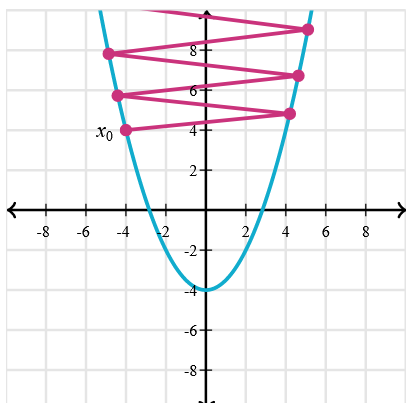
\includegraphics[width = 0.5 \textwidth]{imgs/problem_step_size.png}
    \end{figure}
    
\end{frame}

\begin{frame}{Змінний крок}
    $$x_{k+1} = x_k - \alpha_k \nabla f(x_k), \alpha_k \rightarrow 0$$
    \begin{figure}
        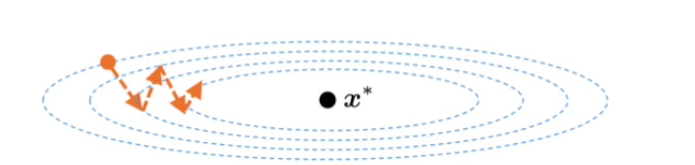
\includegraphics[width = 0.6\textwidth]{imgs/gradient.png}
    \end{figure}
\end{frame}

\begin{frame}{Метод важкого шара Поляка}
    \begin{figure}
        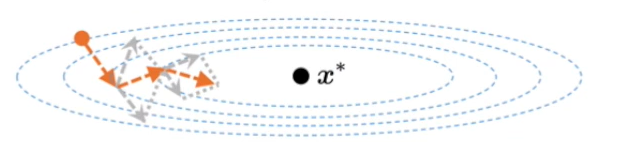
\includegraphics[width = 0.8\textwidth]{imgs/polyak.png}
    \end{figure}
\end{frame}

\begin{frame}{Метод важкого шара Поляка}
    $x_{k + 1} = x_k - \alpha_k \nabla f(x_k) + \beta (x_k - x_{k-1}), 
    \beta $- масса шара 
\end{frame}

\begin{frame}{Метод Нестерова}
    $x_{k + 1} = y_k - \alpha_k \nabla f(y_k) $ 


    $y_{k+1} = x_{k+1} + \beta (x_{k+1} - x_k)$
    \begin{figure}
        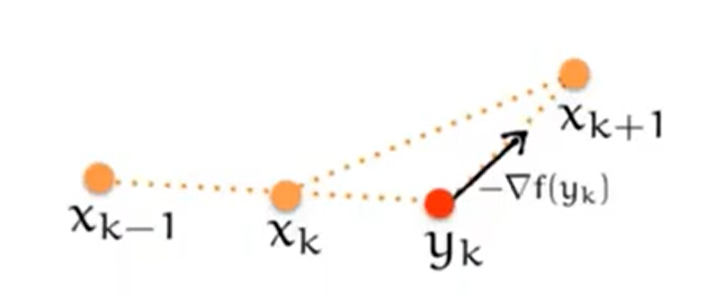
\includegraphics[width = 0.5\textwidth]{imgs/nesterov.png}
    \end{figure}
\end{frame}

\begin{frame}{Метод Нестерова}
    \begin{theo}{Теорема}
        Для досягнення точності $\varepsilon$, отримання 
        $x_N$, такого що $f\left(x_N\right)-f^* \leq \varepsilon$, 
        методу Нестерова потрібно
        
        
        - в опулому випадку: 
        $N=O\left(\frac{L R^2}{\sqrt{\varepsilon}}\right)$


        - у сильно опуклому випадку 
        $N=O\left(\sqrt{\frac{L}{\mu}} \log 
        \left(\frac{1}{\varepsilon}\right)\right)$ 
    \end{theo}
\end{frame}

\end{document}